\documentclass[tikz,border=5pt]{standalone}
\usepackage{tikz}
\usetikzlibrary{positioning,arrows.meta,shapes.geometric,calc}

\begin{document}
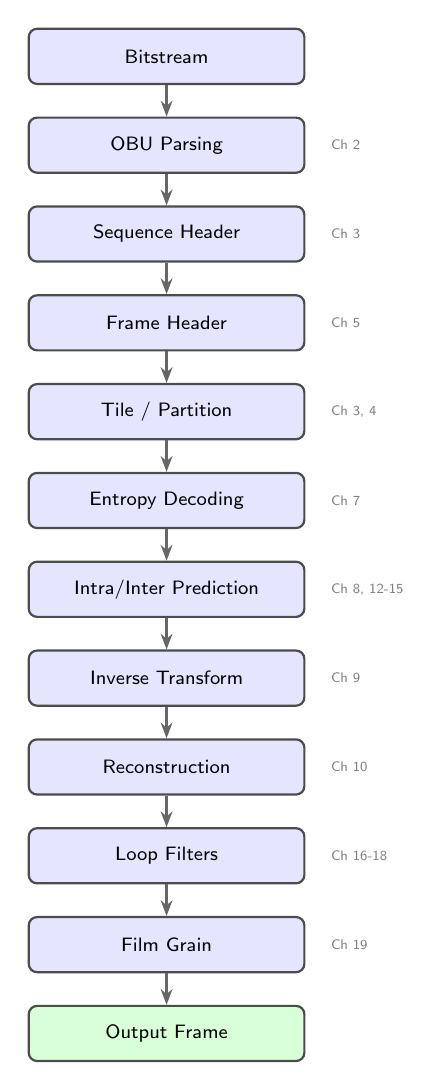
\begin{tikzpicture}[
    stage/.style={draw=black!70, thick, rounded corners=3pt, minimum width=3.5cm, minimum height=0.7cm, fill=blue!10, font=\scriptsize\sffamily},
    arrow/.style={-{Stealth[length=2mm]}, thick, black!60},
    chapter/.style={font=\tiny\sffamily, text=black!50, right=0.2cm}
]

\node[stage] (bitstream) at (0, 0) {Bitstream};
\node[stage, below=0.4cm of bitstream] (obu) {OBU Parsing};
\node[stage, below=0.4cm of obu] (seq) {Sequence Header};
\node[stage, below=0.4cm of seq] (frame) {Frame Header};
\node[stage, below=0.4cm of frame] (tile) {Tile / Partition};
\node[stage, below=0.4cm of tile] (entropy) {Entropy Decoding};
\node[stage, below=0.4cm of entropy] (pred) {Intra/Inter Prediction};
\node[stage, below=0.4cm of pred] (transform) {Inverse Transform};
\node[stage, below=0.4cm of transform] (recon) {Reconstruction};
\node[stage, below=0.4cm of recon] (filter) {Loop Filters};
\node[stage, below=0.4cm of filter] (grain) {Film Grain};
\node[stage, below=0.4cm of grain, fill=green!15] (output) {Output Frame};

% Arrows
\foreach \a/\b in {bitstream/obu, obu/seq, seq/frame, frame/tile, tile/entropy, entropy/pred, pred/transform, transform/recon, recon/filter, filter/grain, grain/output} {
    \draw[arrow] (\a) -- (\b);
}

% Chapter labels
\node[chapter] at (obu.east) {Ch 2};
\node[chapter] at (seq.east) {Ch 3};
\node[chapter] at (frame.east) {Ch 5};
\node[chapter] at (tile.east) {Ch 3, 4};
\node[chapter] at (entropy.east) {Ch 7};
\node[chapter] at (pred.east) {Ch 8, 12-15};
\node[chapter] at (transform.east) {Ch 9};
\node[chapter] at (recon.east) {Ch 10};
\node[chapter] at (filter.east) {Ch 16-18};
\node[chapter] at (grain.east) {Ch 19};

\end{tikzpicture}
\end{document}
